\documentclass[11pt]{article}

\usepackage{enumitem}
\usepackage{amsmath}
\usepackage{amssymb}
\usepackage{bm}
\usepackage{listings}
\usepackage{color}
\usepackage{tikz}
	\usetikzlibrary{shapes,arrows,shadows}
\usepackage[T1]{fontenc}
\usepackage{courier}
\usepackage{circuitikz}
\usepackage{tikz-timing}
    \usetikztiminglibrary{nicetabs}
\usetikzlibrary{calc}
\usepackage{changepage}
\usepackage{multirow}
\usepackage[margin=1.0in]{geometry}
\usepackage[open]{bookmark}

\lstset{xleftmargin=-1cm,
	xrightmargin=\parindent,
    numbersep=5pt} 
    
    \title{CS152B Lab 1}

\definecolor{gray1}{gray}{0.9}
\definecolor{gray2}{gray}{0.8}

\begin{document}
	
\title{\vspace{-0.5in} Com Sci 152B Digital Design \\
	Final Project: Neural Net Digit Identifier }
\date{}
\maketitle
\vspace{-0.75in}
\begin{center}
	\begin{tabular}{cc}
		Michael Hale & 004-620-459 \\ 
		Matthew Nuesca & 904-440-067 \\ 
		Shilin Patel & 904-569-866
	\end{tabular}
\end{center}

\section{Overview}
This final project for CS152B was an open ended exploration of an application of FPGAs. It involved designing and building a product using the knowledge obtained over the quarter. Our goal for this project was to familiarize ourselves with the complexities of building a large multi-function system in Verilog and learn more about the possibilities of programmable hardware.

Our specific project was a convolutional neural network integer identifier trained on the popular MNIST dataset for handwritten digits. The FPGA would train on the data set, continuously updating and optimizing weights. Each 28x28px image would be sent over UART serial from a personal computer. After training is completed, the user may draw an image and send it over serial to be tested on the trained weights. This will then print out the network's inference to a seven segment display. All controls are done without input on the FPGA, but by feeding in different sets of data from the PC, either training data or our test image data.

\section{Background}

Convolutional Neural Networks have proven especially effective at capturing subtle features from image data. However, obtaining optimal weights requires an extensive amount of training. Fortunately the back-propagation algorithm used to train neural networks mostly involves simple, parallelizable operations. In order to improve this process, we designed a system which utilizes specialized hardware resources.

\subsection{Convolutional Neural Networks}

Convolutional Neural Networks are a sub-category of neural networks which combine several layers of linear matrix multiplications paired with non-linear activation functions. As a result, the neural network is very powerful in distinguishing non-linear features. Convolutional Neural Networks combine this principle with the spacial locality inherent in image data. Instead of applying a unique weight to each item in the input vector, a weight filter is instead applied on the image and shifted across the input space. 

{\centering
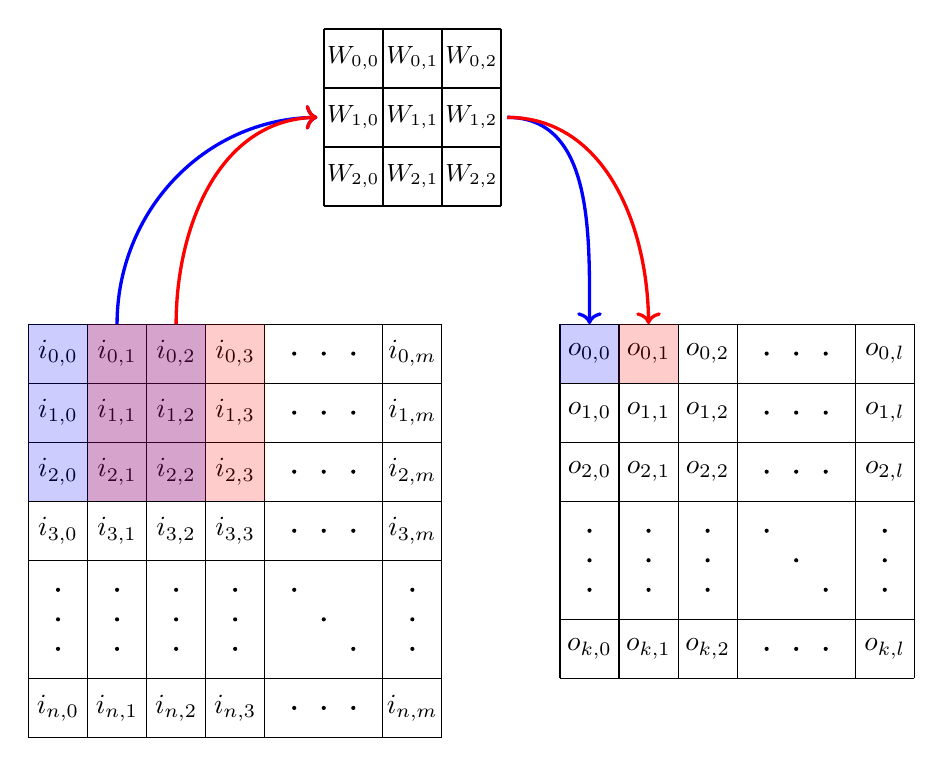
\begin{tikzpicture}[scale=0.75]
\foreach \x in {0,...,4,6,7} {
	\draw[thin] (\x,0) -- (\x,-7);
	\draw[thin] (0,-\x) -- (7,-\x);
}
\foreach \i in {0,1,2} {
	\foreach \j in {0,...,3} {
		\fill (0.5 + \j,-4.5 - 0.5*\i) circle[radius=1pt];
		\fill (4.5 + 0.5*\i,-0.5 - \j) circle[radius=1pt];
	}
	\fill (4.5 + 0.5*\i,-4.5 - 0.5*\i) circle[radius=1pt];
	\fill (6.5,-4.5 - 0.5*\i) circle[radius=1pt];
	\fill (4.5 + 0.5*\i,-6.5) circle[radius=1pt];
}
\foreach \x in {0,...,3} {
	\foreach \y in {0,...,3}
	\draw (0.5 + \x, -0.5 - \y) node[align=center](i-\y-\x) {$i_{\y,\x}$};
	\draw (6.5,-0.5 - \x) node[align=center](i-\x-m) {$i_{\x,m}$};
	\draw (0.5 + \x,-6.5) node[align=center](i-n-\x) {$i_{n,\x}$};
}
\draw (6.5,-6.5) node[align=center] {$i_{n,m}$};

\foreach \x in {0,...,3} {
	\draw[thick] (5,2 + \x) -- (8,2 + \x);
	\draw[thick] (5 + \x,2) -- (5 + \x,5);
}
\foreach \x in {0,1,2}
\foreach \y in {0,1,2}
\draw (5.5 + \x,4.5 - \y) node[align=center](W-\y-\x) {\small{$W_{\y,\x}$}};

\foreach \x in {0,...,3,5,6} {
	\draw[thin] (9 + \x,0) -- (9 + \x,-6);
	\draw[thin] (9,-\x) -- (15,-\x);
}
\foreach \x in {0,1,2} {
	\foreach \y in {0,1,2}
	\draw (9.5 + \x, -0.5 - \y) node[align=center](o-\y-\x) {$o_{\y,\x}$};
	\draw (14.5,-0.5 - \x) node[align=center](o-\x-l) {$o_{\x,l}$};
	\draw (9.5 + \x,-5.5) node[align=center](o-k-\x) {$o_{k,\x}$};
	\foreach \i in {0,1,2} {
		\fill (9.5 + \x,-3.5 - 0.5*\i) circle[radius=1pt];
		\fill (12.5 + 0.5*\i,-0.5 - \x) circle[radius=1pt];
	}
	\fill (12.5 + 0.5*\x,-5.5) circle[radius=1pt];
	\fill (14.5,-3.5 - 0.5*\x) circle[radius=1pt];
	\fill (12.5 + 0.5*\x,-3.5 - 0.5*\x) circle[radius=1pt];
}
\draw (14.5,-5.5) node[align=center](o-k-l) {$o_{k,l}$};
\fill[opacity=0.2, blue] (0,0) rectangle (3,-3);
\fill[opacity=0.2, red] (1,0) rectangle (4,-3);
\draw[->,very thick, blue] (1.5,0) to [out=90,in=180,looseness=1] (W-1-0);
\draw[->,very thick, red] (2.5,0) to [out=90,in=180,looseness=1] (W-1-0);
\fill[opacity=0.2, blue] (9,0) rectangle (10,-1);
\fill[opacity=0.2, red] (10,0) rectangle (11,-1);
\draw[->,very thick,blue] (W-1-2) to [out=0,in=90,looseness=1] (9.5,0);
\draw[->,very thick,red] (W-1-2) to [out=0,in=90,looseness=1] (10.5,0);
\end{tikzpicture} 

Figure 1: Weight filter applied over an input image.\par
}\vspace{11pt}

The diagram above depicts a 3x3 Convolution filter applied to an image with dimensions $n\times m$ with a stride of 1 (meaning the filter is shifter over 1 for each output). If each input $i_{r,t}$ is a vector of depth $p$ and each output is a vector of depth $q$, then each entry in the weight matrix, $W_{x,y}$ is itself a matrix of size $q \times p$. To compute the output $o_{x,y}$ we take the sum over all weights:

$$o_{x,y} = \sum_{r = 0}^2\sum_{t = 0}^2 W_{r,t}i_{r + x,t + y}$$

\subsection{Gradient Descent}
To mathematically optimize the Neural Network, we must apply the gradient descent algorithm to a specific loss function. The principle is to incrementally subtract a fraction of the error gradient from the weights to minimize loss. While training, we are given a correct label for each training sample so during the backpropagation stage we compute an error vector and feed it backwards through the layers of the network. For each layer, we must compute the partial derivative of the error with respect to the input and with respect to the weights. For a fully connected network we compute as follows:
$$\frac{\partial E}{\partial i_t} = \sum_{r=1}^n\frac{\partial E}{\partial o_r} \frac{\partial o_r}{\partial i_t} = \sum_{r=1}^n \delta_r w_{r,t}$$
This is the error vector $\delta$ that we wish to feed into the previous layer and it may be represented as the matrix product:
$$\delta_{in} = W^T\delta_{out}$$
The partial derivative with respect to each weight is just the product of the output error and the input value corresponding to that weight:
$$\frac{\partial E}{\partial w_{r,t}} = i_t\delta_r$$
Once again we may consider the entire weight update as single matrix product:
$$\delta W = i \delta_{out}^T$$
In the case of CNNs, we must isolate each output and input pair when performing updates. For example, when we encounter the output error at coordinate $x,y$ $\delta_{x,y}$, it individually affects all weights but only the inputs at coordinates $x \leq x` < x + K$ where $K$ is the size of the weight filter. 

\subsection{Activation Functions \& Maxpooling}

The activation function is a key component of the neural net, allowing for non-linearity in the model. In our design we chose the popular Rectified Linear (ReLu) activation function. The function simply takes the max of the input or 0, so in hardware it was quite simple to implement since we need only check the sign bit. 

One technique used to reduce the amount of computation required without sacrificing too much performance is max-pooling. Instead of feeding every output from the previous layer into the next layer, we take the max from a small region (say 2x2). Both of these are rather simple manipulations so they are implemented as a part of each layer. 

\section{Design}

Our Verilog design incorporated UART modules, a seven segment display module, a top-level control module, and the core of the design: the neural network layers. The seven segment display plugged into one of the PMOD ports on the Genesys board and was used to display predictions during testing and demonstration. The UART modules enabled the system to communicate to a Python application through an RS-232 cable. \\
 
\tikzstyle{sensor}=[draw, fill=blue!20, text width=5em, 
text centered, minimum height=2.5em,drop shadow]
\tikzstyle{wa} = [sensor, text width=10em, fill=red!20, 
minimum height=6em, rounded corners, drop shadow]
\tikzstyle{conv} = [wa, fill=green!20,text width=5em,minimum height=4em]

{\centering
\begin{tikzpicture}
	\draw (0,0) node[wa] (TLM) {Top Level Module};
	\draw (-4.5,-4) node[conv] (Cone) {Conv 1 Layer};
	\draw (-1.5,-4) node[conv] (Ctwo) {Conv 2 Layer};
	\draw (1.5,-4) node[conv] (DL) {Dense Layer};
	\draw (4.5,-4) node[conv] (SL) {Softmax Layer};
	
	\draw (-4.5,-6) node[sensor] (BA) {Memory Cores};
	\draw (-1.5,-6) node[sensor] (BB) {Memory Cores};
	\draw (1.5,-6) node[sensor] (BC) {Memory Cores};
	\draw (0,-2.4) node[sensor] (BD) {Input Image};
	
	\draw (-4,0) node[conv] (sev-seg) {7 Segment Display};
	\draw (4,0.5) node[conv, minimum height=2em] (UR) {UART Rx};
	\draw (4,-0.5) node[conv, minimum height=2em] (UT) {UART Tx};
	
	\draw[->,thick] (TLM) -- (sev-seg);
	\draw[->,thick] (TLM) to [out=235, in=90, looseness=1] (Cone);
	\draw[->,thick] (TLM.east)+(0,-0.5) -- (UT);
	\draw[->,thick] (SL) to [out=90, in=315, looseness=1] (TLM);
	\draw[<-,thick] (TLM.east)+(0,0.5) -- (UR);
	\draw[->,thick] (Cone) -- (Ctwo);
	\draw[->,thick] (Ctwo) -- (DL);
	\draw[->,thick] (DL) -- (SL);
	\draw[->,thick] (Cone.south)+(-0.5,0) -- +(-0.5,-0.7);
	\draw[<-,thick] (Cone.south)+(0.5,0) -- +(0.5,-0.7);
	\draw[->,thick] (Ctwo.south)+(-0.5,0) -- +(-0.5,-0.7);
	\draw[<-,thick] (Ctwo.south)+(0.5,0) -- +(0.5,-0.7);
	\draw[->,thick] (DL.south)+(-0.5,0) -- +(-0.5,-0.7);
	\draw[<-,thick] (DL.south)+(0.5,0) -- +(0.5,-0.7);
	\draw[->,thick] (TLM.south)+(-0.5,0) -- +(-0.5,-0.7);
	\draw[<-,thick] (TLM.south)+(0.5,0) -- +(0.5,-0.7);
\end{tikzpicture} 

Figure 2: Block diagram of Verilog design. \par
}

\subsection{UART Modules}
There are actually two separate modules for RX and TX communications. It works by instantiating the modules and providing ready bits for when data can be read or written. Once these bits are flipped, the serial communication can begin. Writing out is a simple process of assigning to an output register, while reading places read data on a wire to be moved somewhere for use. These modules are not unique to any other serial uart implementation on an FPGA board. We only had to make minor adjustments in integration with our top module when using a standard serial module.

\subsection{Seven Segment Display}
This module is rather simple. A custom clock is divided from the master clock to ensure the refresh rate of the display is proper for the user to see the shown digit. The module allows the user to input a digit in binary and this will be printed using the PMOD specification detailed the specification.

\subsection{Fixed Point}
Fixed point modules are for performing fixed point operations. They can perform multiplication, addition, division, subtraction. These were built to take two inputs and provide a single output with the correctly formatted fixed point byte size. Fixed point numbers are represented by 32 bits where 15 bits are fractional numbers, 16 bits are integers, and 1 bit is signed. All of these calculations are done using sequential logic. One of the main uses of our fixed point modules is to calculate exponentiation for fixed point numbers. Due to the limit number of multipliers on the FPGA, our implementation consists of a state machine which latches, calculates, then combines the results. During the latch state we ensure that the value does not overflow. We then calculate both fractional and integer parts of the fixed point module and then combine them into one 32 bit piece of data.

\subsection{Python Application}
On the personal computer two python scripts were created, one for training and one for testing. The training script loads the MNIST dataset of 60,000 28x28 greyscale images and attempts to connect to the serial module on the FPGA using the pyserial library. Once a connection is established and the FPGA sends a signal that it is ready to receive one image, the script sends one of the 60,000 images in the dataset along with the corresponding label value (information about which digit is drawn) concatenated to the bytearray. 
For the testing portion of the python implementation the goal was to allow the user to draw a digit on a canvas and then obtain the bytearray and send it serially for testing. To do this required the use of python libraries Tkinter and Pillow which allow a canvas to be drawn upon and the resulting image saved resized and formatted into a 28x28 bytearray.

\subsection{Network Architecture}
Our network utilized two convolutional layers, one fully connected layer, one maxpool layer, and finally a softmax was computed on the output. The 28x28 input vector is expanded to 8x24x24 after the first convolutional layer which utilizes a 5x5 weight filter with a stride of 1. The 2x2 maxpool layer reduces this to a 8x12x12 volume for the second layer. The next convolutional layer also has a 5x5 weight filter and stride of 1, but has an output depth of 16, creating a 16x8x8 output vector. The last dense layer takes this 1024 element vector and computes 10 values which are normalized with softmax to obtain probabilities. 

{\centering
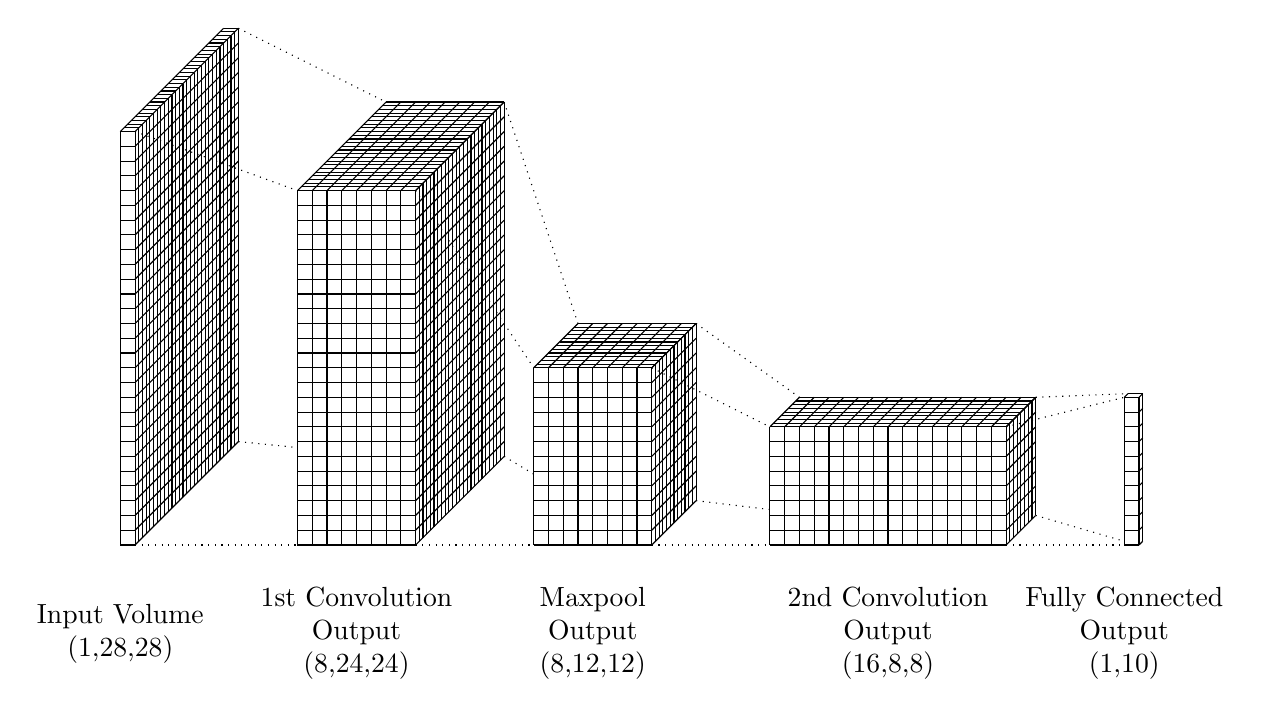
\begin{tikzpicture}[scale=0.75]
\draw[thin] (0,0) -- (0,0.25*28);
\draw[thin] (0,0.25*28) -- (0.25*7,0.25*35);
\foreach \x in {0,...,28} {
	\draw[thin] (0,0.25*\x) -- (0.25,0.25*\x);
	\draw[thin] (0.0625*\x,0.25*28 + 0.0625*\x) -- (0.25 + 0.0625*\x,0.25*28 + 0.0625*\x);
	\draw[thin] (0.25,0.25*\x) -- (0.25*8,0.25*7 + 0.25*\x);
	\draw[thin] (0.25 + 0.0625*\x,0.0625*\x) -- (0.25 + 0.0625*\x,0.25*28 + 0.0625*\x);
}

\foreach \x in {0,...,24} {
	\draw[thin] (3,0.25*\x) -- (5,0.25*\x);
	\draw[thin] (3 + 0.0625*\x,6 + 0.0625*\x) -- (5 + 0.0625*\x,6 + 0.0625*\x);
	\draw[thin] (5,0.25*\x) -- (6.5,1.5 + 0.25*\x);
	\draw[thin] (5 + 0.0625*\x,0.0625*\x) -- (5 + 0.0625*\x,6 + 0.0625*\x);
}
\foreach \x in {0,...,8} {
	\draw[thin] (3 + 0.25*\x,0) -- (3 + 0.25*\x,0.25*24);
	\draw[thin] (3 + 0.25*\x,6) -- (4.5 + 0.25*\x,7.5);
}

\foreach \x in {0,...,12} {
	\draw[thin] (7,0.25*\x) -- (9,0.25*\x);
	\draw[thin] (7 + 0.0625*\x,3 + 0.0625*\x) -- (9 + 0.0625*\x,3 + 0.0625*\x);
	\draw[thin] (9,0.25*\x) -- (9.75,0.75 + 0.25*\x);
	\draw[thin] (9 + 0.0625*\x,0.0625*\x) -- (9 + 0.0625*\x,3 + 0.0625*\x);
}
\foreach \x in {0,...,8} {
	\draw[thin] (7 + 0.25*\x,0) -- (7 + 0.25*\x,3);
	\draw[thin] (7 + 0.25*\x,3) -- (7.75 + 0.25*\x,3.75);
}

\foreach \x in {0,...,8} {
	\draw[thin] (11,0.25*\x) -- (15,0.25*\x);
	\draw[thin] (11 + 0.0625*\x,2 + 0.0625*\x) -- (15 + 0.0625*\x,2 + 0.0625*\x);
	\draw[thin] (15,0.25*\x) -- (15.5,0.5 + 0.25*\x);
	\draw[thin] (15 + 0.0625*\x,0.0625*\x) -- (15 + 0.0625*\x,2 + 0.0625*\x);
}
\foreach \x in {0,...,16} {
	\draw[thin] (11 + 0.25*\x,0) -- (11 + 0.25*\x,2);
	\draw[thin] (11 + 0.25*\x,2) -- (11.5 + 0.25*\x,2.5);
}

\foreach \x in {0,...,10} {
	\draw[thin] (17,0.25*\x) -- (17.25,0.25*\x);
	\draw[thin] (17.25,0.25*\x) -- (17.3125,0.0625 + 0.25*\x);
}
\draw[thin] (17,0) -- (17,2.5);
\draw[thin] (17.25,0) -- (17.25,2.5);
\draw[thin] (17.3125,0.0625) -- (17.3125,2.5625);
\draw[thin] (17,2.5) -- (17.0625,2.5625);
\draw[thin] (17.0625,2.5625) -- (17.3125,2.5625);

\draw[thin, dotted] (0.25,0) -- (3,0);
\draw[thin, dotted] (0.25,28*0.25) -- (3,6);
\draw[thin, dotted] (2,28*0.3125) -- (4.5,7.5);
\draw[thin, dotted] (2,1.75) -- (3,1.65);

\draw[thin, dotted] (5,0) -- (7,0);
\draw[thin, dotted] (5,6) -- (7,3);
\draw[thin, dotted] (6.5,1.5) -- (7,1.2);
\draw[thin, dotted] (6.5,7.5) -- (7.75,3.75);

\draw[thin, dotted] (9,0) -- (11,0);
\draw[thin, dotted] (9,3) -- (11,2);
\draw[thin, dotted] (9.75,0.75) -- (11,0.6);
\draw[thin, dotted] (9.75,3.75) -- (11.5,2.5);

\draw[thin, dotted] (15,0) -- (17,0);
\draw[thin, dotted] (15,2) -- (17,2.5);
\draw[thin, dotted] (15.5,2.5) -- (17.0625,2.5625);
\draw[thin, dotted] (15.5,0.5) -- (17,0.0625);

\draw (0,-1.5) node[align=center] {Input Volume\\(1,28,28)};
\draw (4,-1.5) node[align=center] {1st Convolution\\Output\\(8,24,24)};
\draw (8,-1.5) node[align=center] {Maxpool\\Output\\(8,12,12)};
\draw (13,-1.5) node[align=center] {2nd Convolution\\Output\\(16,8,8)};
\draw (17,-1.5) node[align=center] {Fully Connected\\Output\\(1,10)};
\end{tikzpicture}

Figure 3: Convolutional Neural Network topology. \par
}
\vspace{11pt}

When trained using fixed size gradient descent on a simple python implementation, the network acheived 98\% accuracy on the MNIST test dataset.

\subsection{Neural Network Layers}

The fully connected and convolutional layers were implemented as state machines that would directly feed computations into eachother without the intervention of a control module. Once the first layer has read in all of the inputs and performed its computation, it begins sending data to the next layer and so on. Since we were limited by the number of DSP slices on the Virtex-5, we may only perform a low amount of multiplications in a single cycle. As a result, we must frequently halt the flow of data between the layers while all of the values are computed. \\

{\centering
\begin{tikztimingtable}[
	timing/coldist=2pt,
	timing/nice tabs,
	timing/d/background/.style={fill=white}]
	{\texttt{clk}} & [C] 20{0.5C}; [dotted] 6{0.5C}; 16{0.5C} \\
	{\texttt{o\_valid}} & 3HLL5H; [dotted] HHH; HHLLHHHH \\
	{\texttt{i\_ready}} & 2LH7L; [dotted] LLL;  LHLLLLLL\\
	{\texttt{o\_data}} & 5D{15.76}12D{0.92}4D{-0.11}; \\
	{\texttt{o\_y}} & 5D{11}12D{0}4D{1} \\
	{\texttt{o\_x}} & 5D{0}12D{1}4D{1} \\
	{\texttt{o\_idx}} & 5D{0}12D{0}4D{0} \\
	\extracode
	\tableheader{Signals}{Data Exchange Between Convolution Layers}
	\tablerules
	\begin{pgfonlayer}{background}
		\begin{scope}[gray,dotted,semithick]
			\foreach \x in {0,...,10,13,14,...,20}
			\draw (\x,1) -- (\x,-10.5);
		\end{scope}
	\end{pgfonlayer}
\end{tikztimingtable}

Figure 4: Data exchange timing diagram. \par
}
\vspace{5pt}

The timing diagram above illustrates this idea, where \texttt{o\_valid} is high when the output data from the previous layer is ready and \texttt{i\_ready} is asserted when the next layer is ready to receive input. When both signals are high at the same time, a value has been exchanged between the layers. \texttt{o\_valid} is pulled down while the previous layer reads one of its computed values from memory and updates its outputs: \texttt{o\_data}, \texttt{o\_x}, \texttt{o\_y}, and \texttt{o\_idx}. The last three outputs refer to the specific coordinates and index of the data on the \texttt{o\_data} port. \\

{\centering
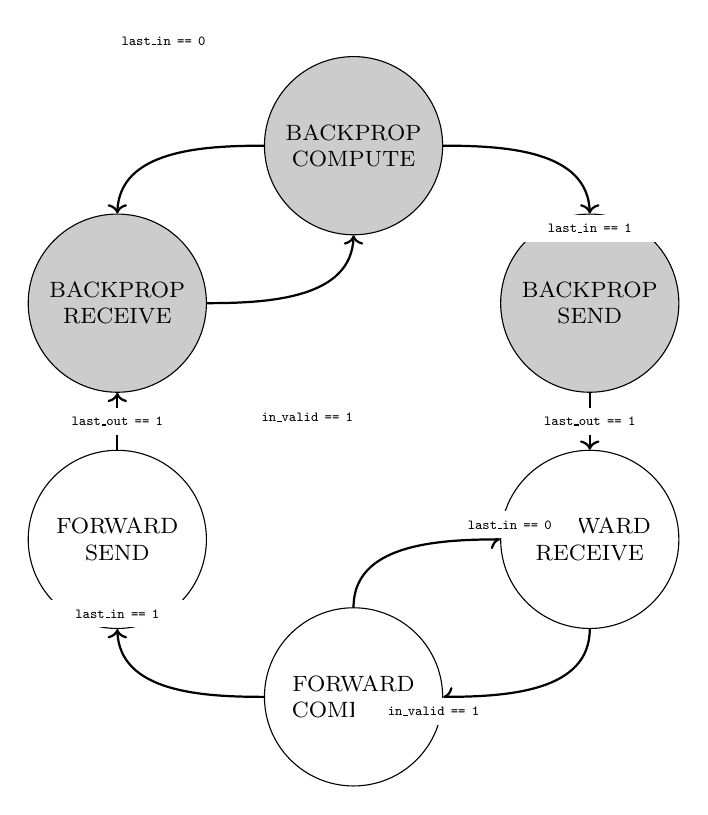
\begin{tikzpicture}
    \path (0,0) node[fill=white,circle,align=center,text width=0.75in,draw,font=\footnotesize] (fw-send) {FORWARD SEND};
    \path (3,-2) node[fill=white,circle,align=center,text width=0.75in,draw,font=\footnotesize](fw-comp) {FORWARD COMPUTE};
    \path (6,0) node[fill=white,circle,align=center,text width=0.75in,draw,font=\footnotesize](fw-rec) {FORWARD RECEIVE};
    \path (0,3) node[fill=gray2,circle,align=center,text width=0.75in,draw,font=\footnotesize](bp-rec) {BACKPROP RECEIVE};
    \path (3,5) node[fill=gray2,circle,align=center,text width=0.75in,draw,font=\footnotesize](bp-comp) {BACKPROP COMPUTE};
    \path (6,3) node[fill=gray2,circle,align=center,text width=0.75in,draw,font=\footnotesize](bp-send) {BACKPROP SEND};

    \draw[->, thick] (fw-rec) to [out=270, in=0, looseness=1] (fw-comp) node[fill=white, font=\tiny,right=0.4in,below=0.0in, text width=0.7in, text centered] {\texttt{in\_valid == 1}};
    \draw[->, thick] (fw-comp) to [out=180,in=270,looseness=1] (fw-send) node[fill=white, font=\tiny, below=0.3in, text width=0.6in, text centered] {\texttt{last\_in == 1}};
    \draw[->, thick] (fw-comp) to [out=90, in=180, looseness=1] (fw-rec) node[fill=white, font=\tiny, left=0.4in,above=0.0in, text width=0.6in, text centered] {\texttt{last\_in == 0}};
    \draw[->, thick] (fw-send) -- (bp-rec) node[fill=white, font=\tiny, midway, text width=0.8in, text centered] {\texttt{last\_out == 1}};
    \draw[->, thick] (bp-rec) to [out=0, in=270, looseness=1] (bp-comp) node[fill=white, font=\tiny, left=0.95in,above=0.45in, text width=0.6in, text centered] {\texttt{last\_in == 0}};
    \draw[->, thick] (bp-comp) to [out=180, in=90, looseness=1] (bp-rec) node[fill=white, font=\tiny, right=0.95in,below=0.5in, text width=0.8in, text centered] {\texttt{in\_valid == 1}};
    \draw[->, thick] (bp-comp) to [out=0, in=90, looseness=1] (bp-send) node[fill=white, font=\tiny, above=0.3in, text width=0.6in, text centered] {\texttt{last\_in == 1}};
    \draw[->, thick] (bp-send) -- (fw-rec) node[fill=white, font=\tiny, midway, text width=0.8in, text centered] {\texttt{last\_out == 1}};
\end{tikzpicture}

Figure 5: State diagram for the convolutional and fully connected layers \par 
}
\vspace{11pt}

The states for the forward stage and backward stage are symmetric, consisting of a receiving, computing, and sending state. The layer waits in the receiving state with its \texttt{o\_ready} pin high until it receives an input, at which point it reads the relevant data from the weights memory block and output value memory block before immediately going into the computing state. 

In the computing state the layer continuously reads from and writes to the output value memory block for each weight that corresponds to the input coordinate and index. Since inputs for a convolution only affect a set number of outputs, upon receiving an input at coordinate $x,y$, we must only update the outputs in the coordinate range $x - k \leq x' < x,y - k \leq y' < y$ where $k$ is the size of the weight filter. The timing diagram below shows the waveforms for computing the forward values. Each requires 3 clock cycles since we must issue a read the first cycle, the second cycle we may access the current value stored in the output block, and the third cycle is when the write back to that address occurs. \\

{\centering
\begin{tikztimingtable}[
    timing/rowdist=20pt,
    timing/xunit=15pt,
    timing/nice tabs,
    timing/d/background/.style={fill=white}]
{\texttt{clk}} & [C] 40{0.5C} \\
{\texttt{o\_valid}} & HHHLL15H \\
{\texttt{conv\_data}} & 5D{0.61}15D{0.05} \\
{\texttt{i\_ready}} & 2LH17L\\
{\texttt{out\_addr}} & 3U 3D{0x000}3D{0x001}3D{0x002}3D{0x010}3D{0x011}2D{0x012} \\
{\texttt{wt\_addr}} & 3U 3D{0x22}3D{0x21}3D{0x20}3D{0x12}3D{0x11}2D{0x10} \\
{\texttt{out\_odata}} & 4U 2D{0.11}1D{0.37}2D{-0.71}1D{-1.36}2D{0.28}1D{0.84}2D{1.99}1D{2.42}2D{-0.34}1D{0.04}1D{0.55} \\
{\texttt{wt\_odata}} & 4U 3D{0.42}3D{-1.06}3D{0.92}3D{0.70}3D{0.62}1D{-0.87} \\
{\texttt{out\_idata}} & 5U 3D{0.37}3D{-1.36}3D{0.84}3D{2.42}3D{0.04} \\
{\texttt{out\_we}} & 5LHLLHLLHLLHLLHLL \\
\extracode
    \tableheader{Signals}{Convolution Forward Computation}
    \tablerules
    \begin{pgfonlayer}{background}
        \begin{scope}[gray,dotted,semithick]
            \foreach \x in {0,...,20}
            \draw (\x,1) -- (\x,-16);
        \end{scope}
    \end{pgfonlayer}
\end{tikztimingtable}

Figure 6: Timing diagram for memory accesses in the forward stage of computation. \par
}
\vspace{11pt}

Once the layer has finished its computation, it will return to the receiving state unless it has just performed computation for the last input value. In that case, it will proceed to the sending state where it will send all its computed values. In the sending state is where the maxpooling and ReLu activation occurs. The layer will read from all the computed values and select the max from those values or 0 if they are all negative. Once this completes, the layer enters the receiving state, but in the backpropagation stage. 

\subsection{Block Memory Cores}

Each convolutional and fully connected layer requires four block memory cores to store different forms of data: the weights, the stored input value, the computed output value, and the computed error value. Since we must access multiple blocks in the same cycle, we must either separate them into different cores or generate a multi-port core with its address space partitioned into differently sized regions. 

The entire design requires 13 block memory cores generated by the Xilinx CoreGen tool. Four are needed for each net layer while one core must be used to buffer image data coming in from serial. One additional benefit of memory cores is the ability to initialize its contents with an plaintext file. 

\subsection{Softmax}
The softmax output function is the last layer in our CNN, it places our 10 outputs between 0 and 1 with the summation of them equal to 1. More specifically, the softmax function is specified as the following: 
$$softmax(x) = \frac{exp(x)}{\sum_{i = 1}^{Num. of inputs} exp(x_i)}$$


Since there is no support for a fixed-point exponentiation, a fixed point exponentiation module had to be implemented. The fixed-point module used splits the input into the integer portion and the fractional portion. The integer portion is used to count the number of times a fixed-point representation of e had to be multiplied multiple times together. The fractional portion was calculated using a taylor polynomial expansion. Due to the limitations of our fixed-point implementation, the taylor polynomial expansion only used the first 5 terms. The expansion is shown below. 

$$exp(x) = 1 + x + \frac{x^2}{2!} + \frac{x^3}{3!} + \frac{x^4}{4!} + \frac{5^2}{5!}$$

The fractional portion and integer portion would be combined by using a multiplier. The exponentiation module uses a finite state machine to split these different mathematical calculations. The first state is an idle state which indicates whether or not the exponential module is busy. Once an input has been latched, it enters a latch stage which checks for overflow (which saturates to return the highest positive fixed floating point number if the input would overflow) and splits the input into an integer and a fraction. It then moves to the calculation phase which does the multiplies needed for the integer portion and the taylor polynomial. It enters a combine state to combine the calculations found for the integer and fraction calculations before returning the value and moving back to the idle state. 

Originally, the implementation used multipliers in parallel to compute the numerator of the polynomial terms as well as to compute the factorial denominators. Division modules were also used in parallel in order to reduce the time of computation. Unfortunately, this design was non-synthesizable due to the lack of multipliers and LUT space found within the Virtex-5. The module had to be re-written to only use 1 multiplier and 1 division module. Additionally, since the denominators were constant, no multipliers used. Instead, we opted to use a parameter array to hold 5 32 bit numbers concatenated together . This allowed the exponential module and the softmax function to be synthesizable together. 

The softmax layer consists of multiple states as well:
\begin{enumerate}
	\item Receive input
	\item Perform additions and exponentials
	\item Perform divisions
	\item Backpropagation
\end{enumerate}

These states, unlike the design in the conv and FC layers, do not simply transition from the prior to the next. In the receiving input state we determine whether to transition to the computational states or to the backpropagation state. Each of the states in this softmax state machine perform the mathematical requirements of the softmax function, however there are issues with max values and overflow which are handled by the fixed point exponentiation implementation. 

The softmax layer was originally written to have each of the 10 inputs contain its own exponential module to compute the exponents in parallel. While synthesizable, it took a big \% of LUTS as well as 40 out of the 48 DSP slice multipliers found in the FPGA. As a result, the softmax layer to be rewritten to only use 1 exponential module. This would result in a a more space efficient implementation. Due to time constraints, simulation of the implemented module contained many bugs that weren’t able to fixed and could not be integrated with the additional layers. 

\section{Challanges}

This project was unfortunately plagued with issues from conception. Our first proposal was to use DDR2 SDRAM in order to host the MNIST dataset on the board itself. The idea was to simply access the SDRAM instead of constantly checking over serial for the next image to process. The process to initialize the SDRAM took over a week. It began with problems on improper setting of parameters in the xilinx GUI menus. After these issues were resolved and the SDRAM module was created, we ran into the problem of the ready signal not triggering for loading data into the memory. Even after we spent hours pouring over the manual and consulting with others attempting to use the memory, we were forced to look for different methods of handling the dataset, as this module was proving to be too much trouble to initialize properly. We settled on transferring one image at a time over serial and notifying the PC, when sending an image was appropriate with a ready signal from the FPGA serial module. 

Once of the requirements of the convolutional network we were building was the necessity to store inputs, outputs, weights, and error values for prolonged periods of time and have them accessible to each layer. Our first attempt was to simply store all of this data in registers, however it soon became apparent that the LUT would not be able to host all of this information. The solution to this problem was to use the core generator to make BRAM modules. Only after the BRAM was initialized and working it became clear to us that the reset pin that the core generator created did not have consistent behaviour on our Virtex5 product. This resulted in the need to reprogram the board after each test run. An inconvenience for sure, however still usable.

When implementing our CNN layers, especially in the convolutional and fully connected layers our understanding of the arithmetic components of the FPGA were put to the test. We severely overestimated the ability to do multiplication in parallel because we didn’t realize that the FPGA had 48 multipliers. Our previously built implementations of the conv and FC layers would have to be adjusted to multiply sequentially (not in parallel). The solution to this was adjusting one layer to take place over many more clock cycles than previously planned. This actually didn’t have as adverse effects on our training speed as predicted. We would still be able to train on the MNIST dataset in only a few minutes.

Apart from these challenges to do with our lack of information or the complexity of a certain feature, some other challenges faced was the problem of being tied to the lab to do all of our work. Due to our reliance on the core generator and other xilinx tools, we were unable to work and simulate from our personal computers as effectively as other groups. A final odd bug we encountered while testing softmax was an iSim graphical error where the values of the waveform would become invalidated when too much data was viewed through the window. We didn’t understand this was a graphical error and this led to more wasting of precious time. 

In the end our final product was delivered in the form of the test implementation which completed serial, BRAM, testing(w/o softmax), and seven segment portions of the network completed. This allowed for a demo that output a predicted digit from a drawn image. However, the weights were acquired by training on a python implementation of our CNN and then loaded into the BRAM for access during the test run. Our infrastructure for training exists but unresolved errors forced us to abandon it.

\section{Conclusion}

In total, even with all of the difficulties, this project was extremely worthwhile to undergo. We learned in depth about the hardware components associated with the FPGA as well as built in tooling Xilinx provides. Some of us also had to study how CNNs work from the ground up and familiarize ourselves with the formulas and algorithms that build neural networks. Some python library exploration was a bonus experience! It was a rewarding process from start to finish even when nothing worked to the point where only some things worked. If done again, we would definitely want to avoid the time sink that dealing SDRAM was, however in an area without many resources outside of few forum posts and complex official documentation, we believe we achieved a good deal of what we proposed.

\end{document}